Šioje dalyje apmokant tinklą analizuosiu tinklo apmokymą apibūdinančius parametrus:
\begin{enumerate}
  \item Palyginsiu tinklo apmokymo vidutines paklaidas, kai tinklo naujam apmokymui yra naudojamos praeito apmokymo dalinės išvestinės su tinklo apmokymu, kai dalinės išvestinės po kiekvienos apmokymo iteracijos yra nunulinamos.
  \item Lyginsiu tinklo vidutines paklaidas priklausant nuo apmokymų skačiaus su skirtingomis $\alpha$ ir $\eta$ reikšmėms.
  % \item Lyginsiu tinklo apmokymo vidutines paklaidas didėjant apmokymo duomenų kiekiui.
  \item Atliksiu tinklo apmokymo greitaveikos tyrimą, esant skirtingoms tinklo topologijoms.
  % \item Palyginsiu tinklo apmokymo greitį skaičiavimus atliekant ant CPU ir GPU.
\end{enumerate}


\textbf{Tinklo apmokymo vidutinių paklaidų lyginimas, kai naujam tinklo apmokymui yra naudojamos praeito žingsnio dalinės išvestinės su tinklo apmokymu, kai dalinės išvestinės po kiekvieno apmokymo yra nunulinamos.}

Šis tyrimas bus atliekamas prie vienodų tinklo parametrų.
$\alpha = 0.8$
$\eta = 0.2$
Topologija - įvesties h reikšmių bus M, įvesties x reikšmių bus I+1, išvesties reikšmių, taip pat bus M.

Abiejais atvejais bus vykdomas apmokymas atliekant n=100 epochų.

Lyginsime tinklo vidutines paklaidas po kiekvienos apmokymo epochos. (\ref{fig:paklaidos1})

\begin{figure}[h!]
  \centering
\scalebox{0.6}{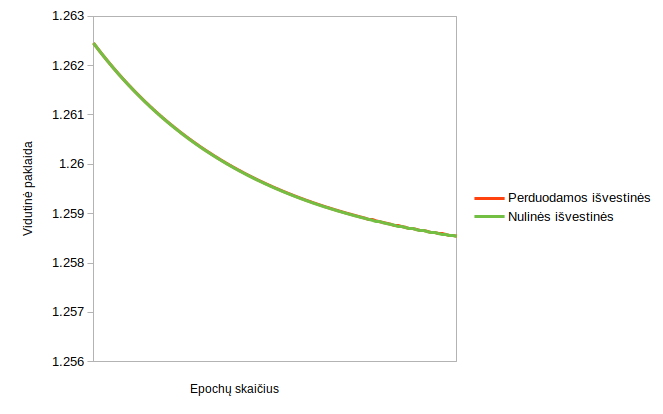
\includegraphics{images/paklaida.png}}
\caption{Apmokymo paklaidos.}
\label{fig:paklaidos1}
\end{figure}

Tinklą apmokant naudojant abu būdus, tinklo apmokymo klaidos funkcijų grafikai yra identiški, todėl nėra būtina šių paklaidų perduoti atliekant naują apmokymą.

\textbf{Lyginsiu tinklo vidutines paklaidas priklausant nuo apmokymų skačiaus su skirtingomis $\alpha$ ir $\eta$ reikšmėms.}
\clearpage
\begin{figure}[h!]
  \centering
\scalebox{0.6}{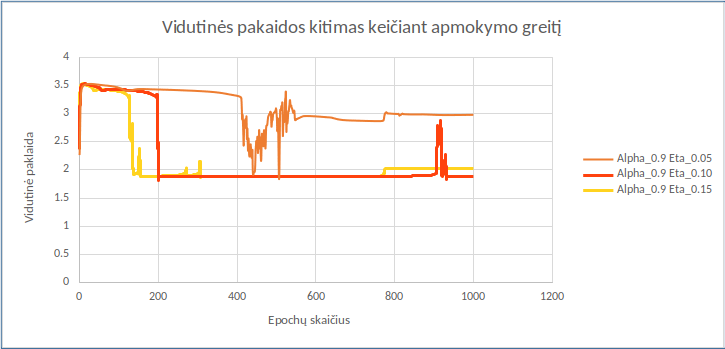
\includegraphics{images/etakitimas.png}}
\caption{Tinklo apmokymo paklaidos grafikas su skirtingais apmokymo greičiais.}
\label{fig:etakitimas}
\end{figure}

Iš grafiko \ref{fig:etakitimas} galima pastebėti, kad tinklas geriausiai apsimoko, kai apmokymo greičio koeficientas $\eta=0.15$, tačiau grafikas gaunasi tiesinis po 200-os epochos, tai galėjo nutikti dėl to, kad funkcija pateko į lokalaus minimumo tašką. Taip pat tinklas panašiai apsimoko, kai apmokymo greičio koeficientas yra $\eta=0.1$, tačiau galima pastebėti, kad ties 950-a epocha yra kažkokių nukrypimų. Kai $\eta=0.05$, tai tinklas apsimoko prasčiausiai, intervale (400;600) grafike taip pat galima pastebėti nukrypimų, tačiau nuo 600-os epochos tinklo vidutinė paklaida ima tolygiai mažėti.


\begin{figure}[h!]
  \centering
\scalebox{0.6}{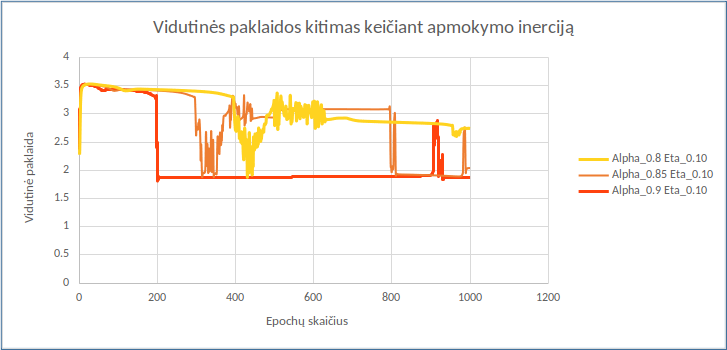
\includegraphics{images/alphakitimas.png}}
\caption{Tinklo apmokymo paklaidos grafikas su skirtingom apmokymo inercijom.}
\label{fig:alphakitimas}
\end{figure}

Iš grafiko \ref{fig:alphakitimas} galima pastebėti, kad tinklas geriausiai apsimoko, kai apmokymo inercijos koeficientas $\alpha=0.9$, tačiau grafikas gaunasi tiesinis po 200-os epochos, tai galėjo nutikti dėl to, kad funkcija pateko į lokalaus minimumo tašką. Tinklas apsimoko panašiai iki 800-os epochos prie koeficientų $\alpha=0.85$ ir $\alpha=0.8$, o ties 400-a epocha yra kažkokių nukrypimų, tačiau nuo 800-os epochos grafikai išsiskiria ir kai $\alpha=0.85$ tinklo apmokymas susilygina su tinklo apmokymu, kai $\alpha=0.9$.

\textbf{Atliksiu tinklo apmokymo greitaveikos tyrimą, esant skirtingoms tinklo topologijoms.}

\begin{figure}[h!]
  \centering
\scalebox{0.6}{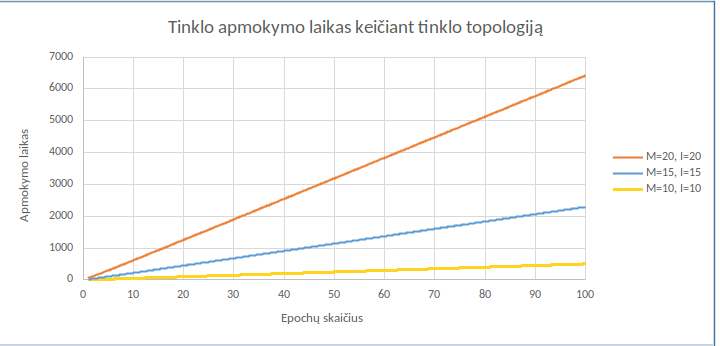
\includegraphics{images/laikograf.png}}
\caption{Tinklo apmokymo laiko palyginimas keičiant tinklo topologijas.}
\label{fig:laikograf}
\end{figure}

Iš grafiko galima pastebėti, kad vidutiniai vienos epochos apmokymo laikai, kai tinklo topologijos yra
\begin{enumerate}
  \item M=10, I=10 (840 svorių) - 5 sekundės.
  \item M=15, I=15 (1860 svorių) - 23 sekundės.
  \item M=20, I=20 (3280 svorių) - 64 sekundės.
\end{enumerate}
Galima pastebėti, kad didinant tinkle esančių svorių kiekį, tinklo apmokymo laikas didėja eksponentiškai.
